\documentclass[a4paper,titlepage,12pt]{article}
\usepackage[utf8]{inputenc}
\usepackage{todonotes}
\usepackage{url}
\usepackage{listings}
\usepackage{color}
\usepackage{subcaption}
\begin{document}
 
\newcommand{\horrule}[1]{\rule{\linewidth}{#1}}     % Horizontal rule

\title{
        %\vspace{-1in}  
        \usefont{OT1}{bch}{b}{n}
        \normalfont \normalsize \textsc{KU Leuven} \\ [25pt]
        \normalfont \normalsize \textsc{Computer Vision} 
        \horrule{2pt} \\[0.5cm]
        \huge Final Project: Incisor Segmentation \\
        \horrule{2pt} \\[0.5cm]
}
\author{
        \normalfont            
        Joran Van de Woestijne (r0378602)\\
        Tim Van Den Broecke (r0296620)
}
\date{August 2017}
 
\maketitle

\newpage
\tableofcontents
\thispagestyle{empty}
\newpage
\setcounter{page}{1}

\section{Introduction}
\todo[inline]{TODO: Joran}

\section{Shape Model}
\todo[inline]{TODO: Tim}

\subsection{Shape alignment}

\subsection{PCA analysis}

\section{Radiograph pre-processing}

Dental radiographs are inherently noisy and contain too much information when just focusing on locating the upper and lower incisors.
For instance, all the teeth (not just the incisors), the jaw and the nose are present in the radiographs.
To reduce these radiographs to a more suitable size for our application, we crop them based on domain knowledge so that only the smaller region around the four incisors remains.

After the size reduction, the radiographs still need to be de-noised so that it's easier for our algorithm to detect the edges.
We achieve this by using the technique proposed in \textit{Noise Removal and Contrast Enhancement for X-Ray Images} by Huang et al \cite{JBEMI1893}.
The algorithm proposed by Huang et al is visualised in Figure \ref{preprocessalgo}. This technique first starts off by applying an adaptive median filter to reduce the impulsive (salt-and-pepper) noise, after which a bilateral filter is used to suppress the Gaussian noise while also preserving the edges of the image.
After the noise suppression step, the radiograph is sharpened by a mathematical morphology, here a top hat and bottom hat transform.
The top hat transform enhances the brighter regions of the radiograph, whereas the bottom hat enhances the darker regions.
Finally, the contrast of the radiograph is enhanced by applying a contrast limited adaptive histogram equalization (CLAHE).
To detect the edges of the dental radiograph, a Sobel operator is used, detecting the gradients in the x and y direction.
The results of applying the different pre-processing steps on a dental radiograph can be observed in Figure \ref{preprocess}. 


\begin{figure}
\centering
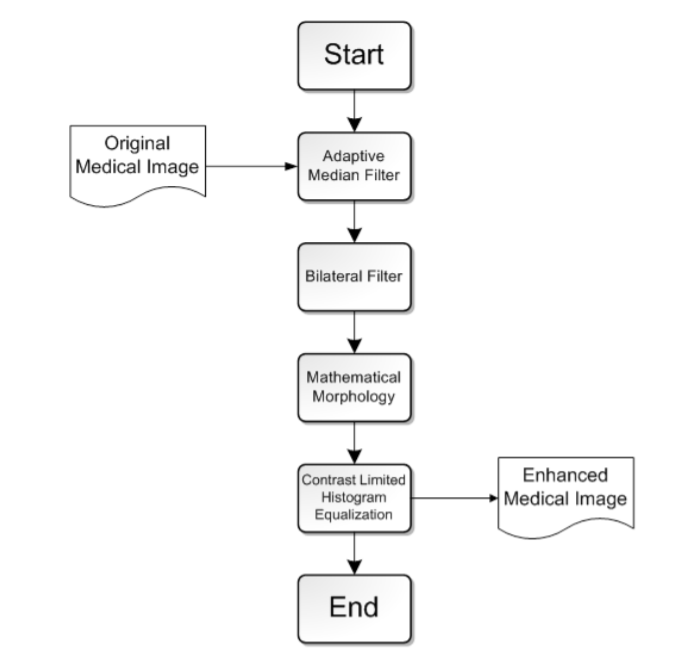
\includegraphics[width=0.7\linewidth]{preprocess/algorithm.png}
  \caption{
		The algorithm proposed by Huang et al \cite{JBEMI1893} for denoising dental radiographs. The algorithm has four steps, with a top hat transform and a bottom hat transform representing the mathematical morphology step. } \label{preprocessalgo}
\end{figure}

\begin{figure}
  \centering
	\begin{minipage}[b]{0.32\linewidth}
		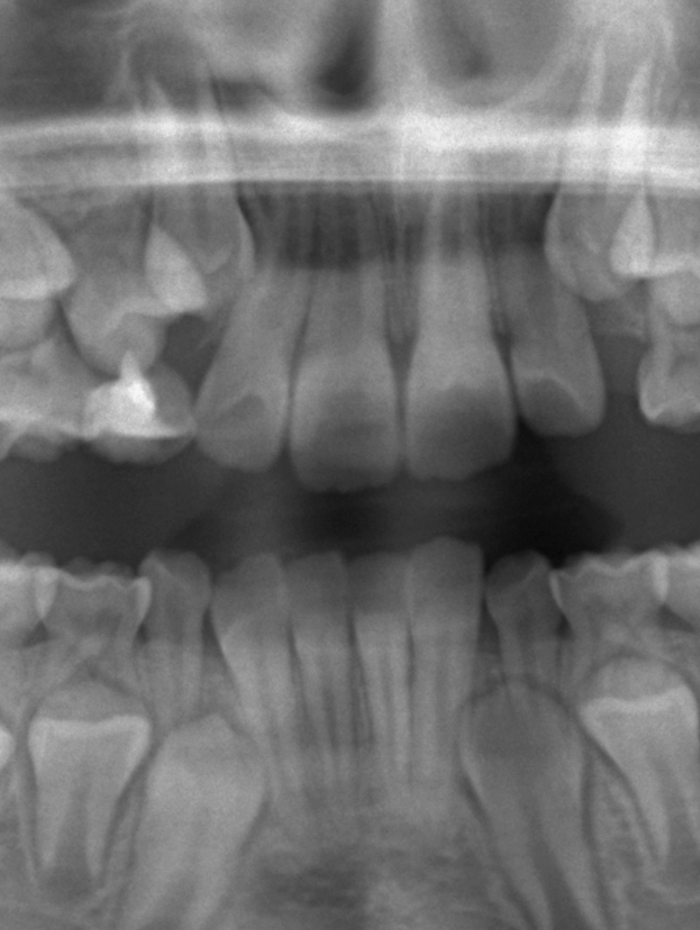
\includegraphics[width=\linewidth]{preprocess/original.png}
		\subcaption{Cropped}
	\end{minipage}
	\begin{minipage}[b]{0.32\linewidth}
		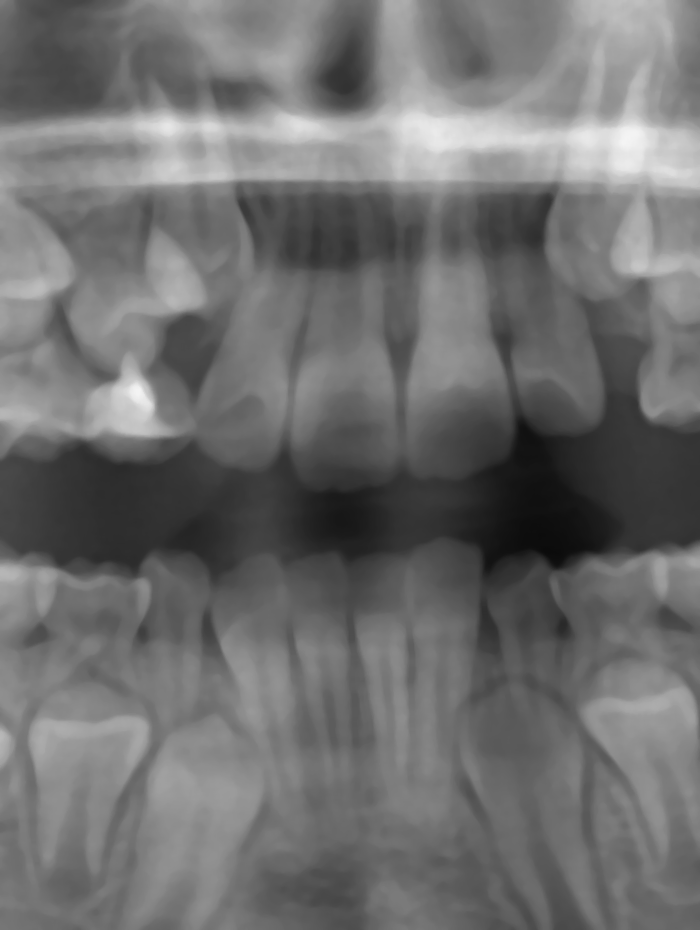
\includegraphics[width=\linewidth]{preprocess/median.png}
		\subcaption{Median filter}
	\end{minipage}
	\begin{minipage}[b]{0.32\linewidth}
		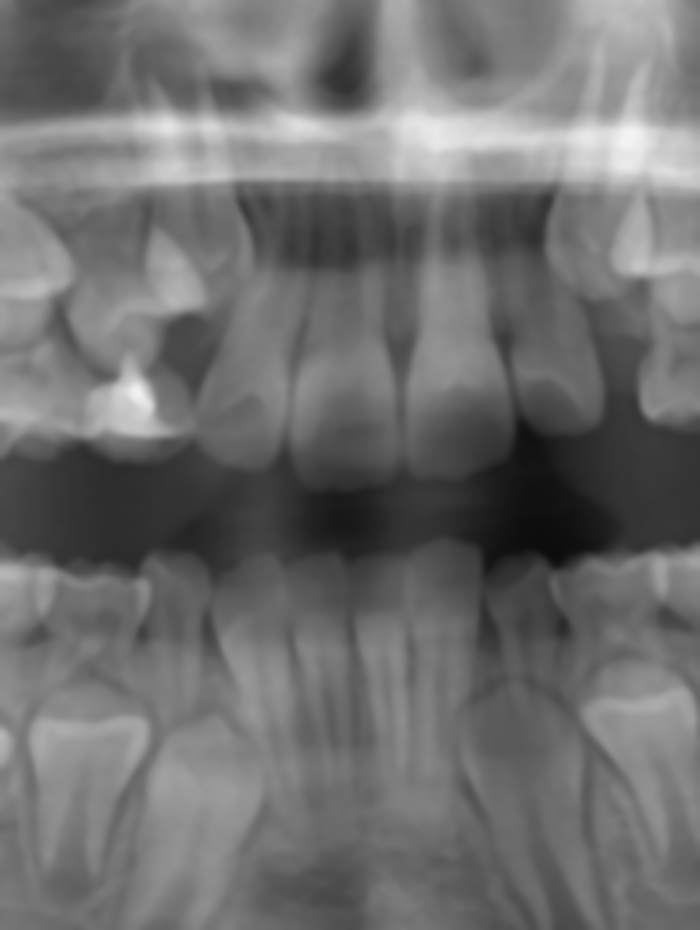
\includegraphics[width=\linewidth]{preprocess/bilateral.png}
		\subcaption{Bilateral Filter}
	\end{minipage}
	\begin{minipage}[b]{0.32\linewidth}
		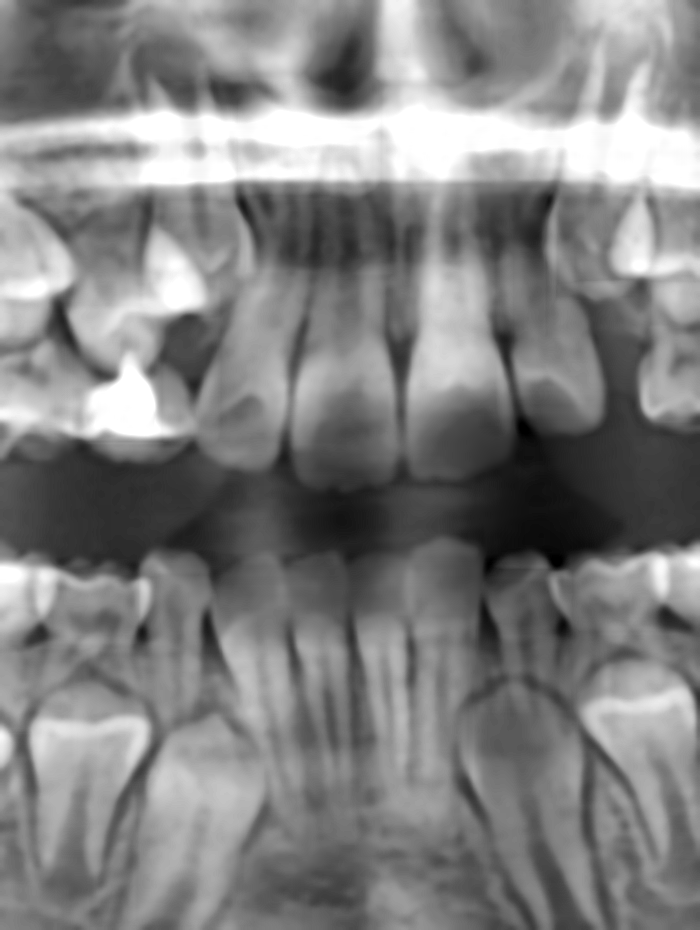
\includegraphics[width=\linewidth]{preprocess/hats.png}
		\subcaption{Top and Bottom hat}
	\end{minipage}
	\begin{minipage}[b]{0.32\linewidth}
		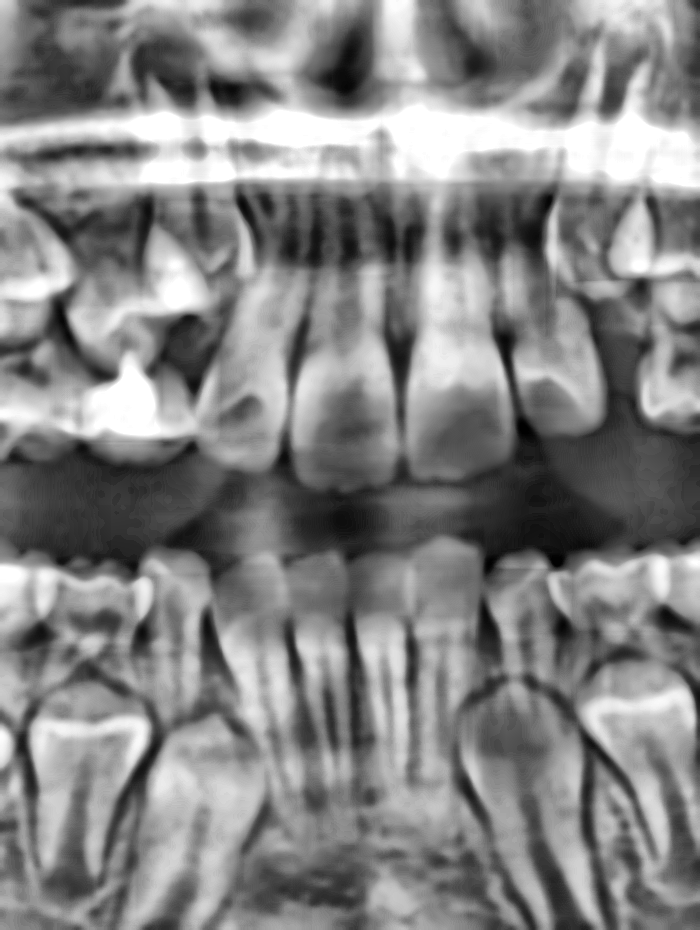
\includegraphics[width=\linewidth]{preprocess/clahe.png}
		\subcaption{CLAHE}
	\end{minipage}
	\begin{minipage}[b]{0.32\linewidth}
		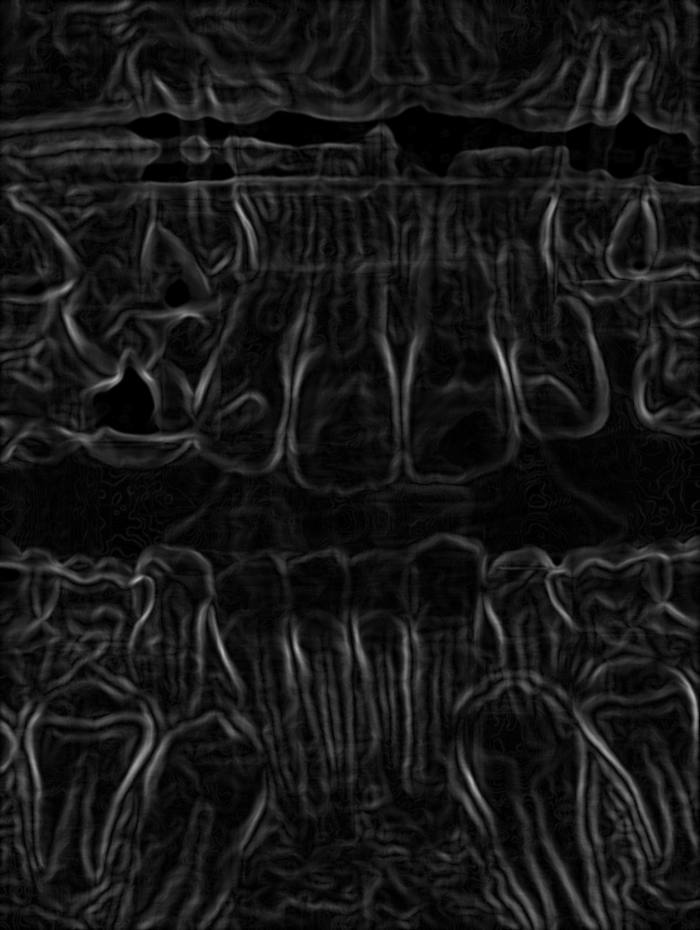
\includegraphics[width=\linewidth]{preprocess/gradients.png}
		\subcaption{Edges (Sobel)}
	\end{minipage}
  \caption{
		The results of the different pre-processing steps visualised when applied on dental radiograph 3.
		(a) shows the original image after cropping, (b) shows (a) after applying the adaptive median filter, (c) adds the bilateral filter onto the result of (b), (d) performs the mathematical morphology (top hat and bottom hat) on (c), and (e) finally applies CLAHE. A Sobel operator is used to detect the edges, which is visualised in (f).} \label{preprocess}
\end{figure}


\section{Fitting model to image}


\subsection{Initial pose estimate}

\begin{figure}
  \centering
	\begin{minipage}[b]{0.32\linewidth}
		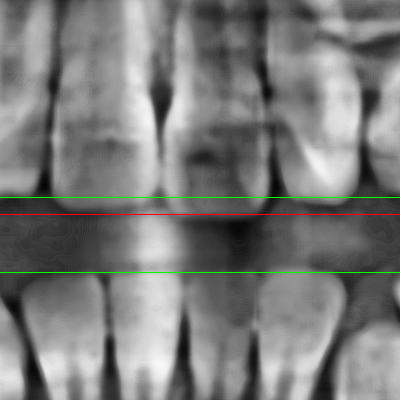
\includegraphics[width=\linewidth]{init/sep.png}
		\subcaption{Jaw separation}
	\end{minipage}
	\begin{minipage}[b]{0.32\linewidth}
		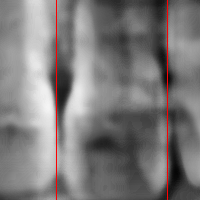
\includegraphics[width=\linewidth]{init/up.png}
		\subcaption{Upper hough lines}
	\end{minipage}
	\begin{minipage}[b]{0.32\linewidth}
		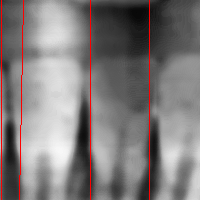
\includegraphics[width=\linewidth]{init/down.png}
		\subcaption{Lower hough lines}
	\end{minipage}
	\begin{minipage}[b]{0.32\linewidth}
		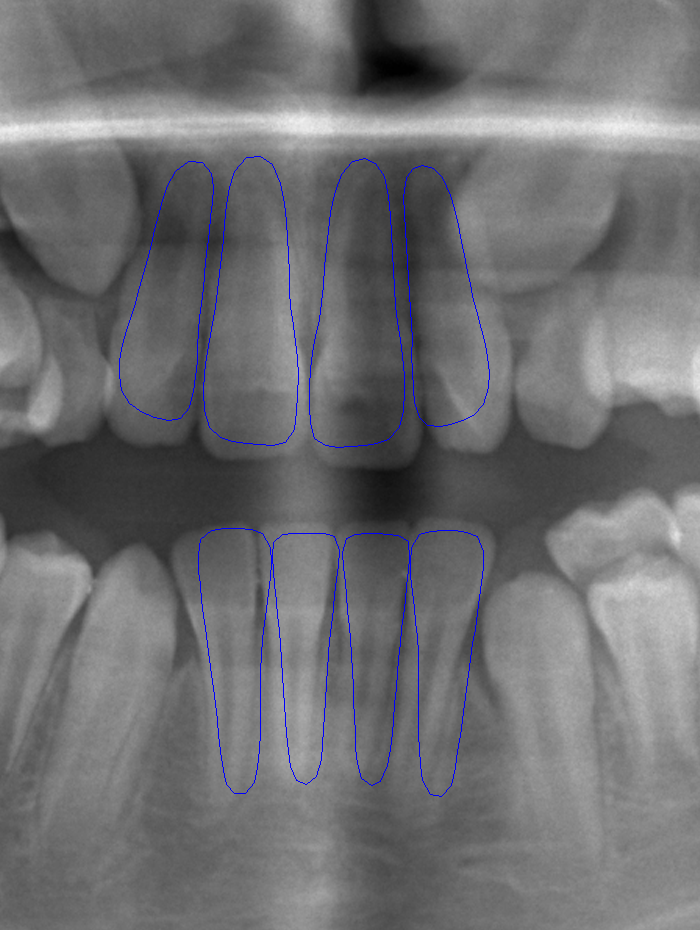
\includegraphics[width=\linewidth]{init/initial.png}
		\subcaption{Result for image 11}
	\end{minipage}
	\begin{minipage}[b]{0.32\linewidth}
		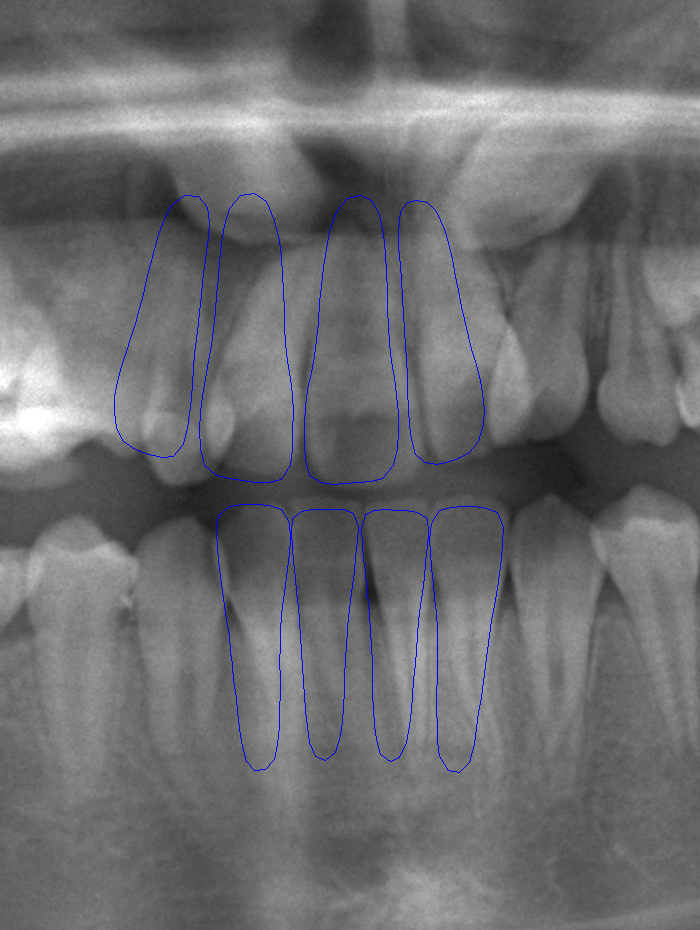
\includegraphics[width=\linewidth]{init/initial6.png}
		\subcaption{Result for image 5}
	\end{minipage}
  \caption{
		The process of getting the initial pose estimate. (a) shows the jaw separation lines for radiograph 11, where the red line shows the row of pixels with the lowest intensity and the green lines show the resulting upper and lower jaw separations.
		(b) and (c) show the hough lines for the upper and lower incisors respectively for radiograph 11.
		(d) shows the resulting initial estimate for radiograph 11, which is a really good fit, and (e) shows the initial estimate for radiograph 3.
		The estimate for radiograph 3 is a lot worse due to the off-centered position of the upper incisors.} \label{init}
\end{figure}

\subsection{The ASM algorithm}

\section{Evaluation}

\todo[inline]{TODO: Tim}

\section{Conclusion}

\todo[inline]{TODO: Tim, if even necessary after evaluation?}

\bibliography{references}
\bibliographystyle{plain}

\end{document}
